\documentclass[12pt,a4paper]{article}

\usepackage{fontspec}
\usepackage{polyglossia}
\setmainlanguage{english}
\setmainfont{Latin Modern Roman}

\usepackage[a4paper,left=2.15cm,right=2.15cm,top=2.05cm,bottom=2.15cm]{geometry}
\usepackage{amsmath,amssymb}
\usepackage{graphicx}
\usepackage{array}
\usepackage{booktabs}
\usepackage{caption}
\usepackage{subcaption}
\usepackage{float}
\usepackage{hyperref}
\usepackage{indentfirst}
\usepackage{ragged2e}

\hypersetup{hidelinks}
\captionsetup{font=small,labelformat=empty,justification=centering}
\setlength{\parindent}{1.15cm}
\setlength{\parskip}{0pt}
\renewcommand{\arraystretch}{1.15}

\newcommand{\chaptertitle}[1]{\section*{#1}\addcontentsline{toc}{section}{#1}}
\newcommand{\subchaptertitle}[1]{\subsection*{#1}\addcontentsline{toc}{subsection}{#1}}
\newcommand{\figcaption}[1]{\caption*{\small #1}}
\newcommand{\twopanel}[4]{%
  \begin{figure}[H]\centering
    \begin{minipage}{0.48\textwidth}\centering
      \includegraphics[width=\linewidth]{#1}\\[-0.2em]a)
    \end{minipage}\hfill
    \begin{minipage}{0.48\textwidth}\centering
      \includegraphics[width=\linewidth]{#2}\\[-0.2em]b)
    \end{minipage}
    \figcaption{#3 #4}
  \end{figure}
}

\begin{document}
\pagestyle{plain}

\begin{titlepage}
\thispagestyle{empty}
\centering
{\large University of Warsaw\\
Faculty of Physics\par}
\vspace{1.4cm}
{\large Bartosz Wieciech\\
student record no.: 276965\par}
\vspace{3.0cm}
{\Large\itshape Modeling light propagation in photonic nanostructures\\
using the finite element method\par}
\vspace{1.7cm}
{\large Bachelor's thesis\\
in nanostructure engineering\\
in the field of photonics\par}
\vfill
\begin{flushright}
Thesis prepared under the supervision of\\
dr hab. Rafał Kotyński\\
Division of Information Optics
\end{flushright}
\vspace{1.6cm}
Warsaw, September 2014
\end{titlepage}

\setcounter{page}{2}
\mbox{}
\newpage

\chaptertitle{Statement of the thesis supervisor}

I declare that this thesis was prepared under my supervision and state that it meets the conditions
for submission in proceedings for the award of a professional degree.

\vspace{1.5cm}
\noindent Date\hspace{3.5cm}Signature of the thesis supervisor

\vspace{2.0cm}
\chaptertitle{Statement of the author}

Aware of legal liability, I declare that this diploma thesis was written by me independently and
does not contain content obtained in a manner inconsistent with applicable regulations.

I also declare that the submitted thesis has not previously been the subject of procedures connected
with obtaining a professional degree at an institution of higher education.

I further declare that this version of the thesis is identical to the attached electronic version.

\vspace{1.5cm}
\noindent Date\hspace{3.5cm}Signature of the author

\newpage
\mbox{}
\newpage

\chaptertitle{Abstract}

The finite element method was applied to model the propagation of light in periodic photonic
nanostructures. For this purpose, a two-dimensional vector wave equation was solved. Simulations
were performed for photonic crystals with different lattice structures, into which linear defects were
introduced. Differences resulting from the use of waves of different frequencies, lying both inside
and outside the photonic band gap of the system, are presented. A simulation of guiding a localized
mode in the linear defect of a photonic crystal was performed. The transmission of electromagnetic
radiation through diffraction gratings with double periodicity was also studied. Modeling was carried
out for systems made of silver, gold, chromium, and a perfect conductor, for a wavelength of 400 nm.

\vspace{1.2cm}
\chaptertitle{Keywords}

Finite element method, electromagnetic modeling, PML, light, vector wave equation, photonic
crystal, photonic band gap, subwavelength grating

\vspace{1.2cm}
\chaptertitle{Field of the thesis (codes according to the Socrates-Erasmus program)}

[13.2] Physics

\vspace{1.2cm}
\chaptertitle{Title of the thesis in English}

Modeling of light propagation in photonic nanostructures using the finite element method

\newpage
\mbox{}
\newpage

\chaptertitle{Contents}
\begingroup\small
\noindent Chapter 1. Introduction\dotfill 8\\
Chapter 2. Theoretical background\dotfill 9\\
\hspace*{1em}2.1. Maxwell equations and the two-dimensional vector wave equation\dotfill 9\\
\hspace*{1em}2.2. Finite element method\dotfill 11\\
\hspace*{1em}2.3. Elliptic differential equation and a method for its approximate solution\dotfill 12\\
\hspace*{1em}2.4. PML boundary conditions\dotfill 13\\
\hspace*{1em}2.5. Photonic crystals\dotfill 15\\
\hspace*{1em}2.6. Diffraction gratings\dotfill 16\\
Chapter 3. Simulation results\dotfill 18\\
\hspace*{1em}3.1. Propagation of light in photonic crystals\dotfill 18\\
\hspace*{1em}3.2. Diffractive elements with double periodicity\dotfill 26\\
Chapter 4. Conclusions\dotfill 29\\
Bibliography\dotfill 30
\endgroup

\newpage

\chaptertitle{Chapter 1. Introduction}

Photonics is a rapidly developing field of science that combines elements of optics, solid-state
physics, materials engineering, computer science, and electronics. The ability to control light has
become extremely important today, among other things for efficient information transfer, more
accurate imaging, and the production of advanced optical filters. The newest discoveries in condensed
matter physics became a starting point for research on the use of semiconductors in optics, which
brought new possibilities that had not been known before. Dielectric micro- and nanostructures,
such as photonic crystals, used by nature for millions of years, have made possible, among other
things, selective guiding and trapping of light, while metal-dielectric systems have become the basis
for the development of plasmonics.

Because of the cost and the difficult-to-predict properties of complex photonic systems, it is
necessary -- in order to obtain the desired properties and optimize them -- to carry out computer
simulations. Well-developed methods for studying light propagation in new materials include, for
example, FEM (finite element method) and FDTD (finite difference time domain method). To
determine the band structure of periodic systems, the PWM method (plane wave method) can be
used. The combination of these methods makes it possible to obtain a wide range of information
about the structure under consideration, which enables possible modifications to improve efficiency
and also to find new potential applications.

This thesis is based on the finite element method, one of the methods for solving differential
equations and an extremely useful tool for modeling the behavior of electromagnetic waves in
photonic structures. It was used to study light propagation in photonic crystals with different lattice
types and different sizes. It was also applied to determine the properties of diffractive elements with
double periodicity, depending on the direction from which the structure is illuminated and on the
material from which it is made.

In summary, the use of computer modeling to design new nano-optical systems is an important
problem that enables the production of modern photonic devices. The foundations of finite element
method simulations, supplemented by the finite difference time domain method and the plane wave
method, are presented in this thesis.

\newpage
\chaptertitle{Chapter 2. Theoretical background}

\subchaptertitle{2.1. Maxwell equations and the two-dimensional vector wave equation}

Electromagnetic fields in vacuum are uniquely described by the four Maxwell equations, whose
differential form is:
\begin{align}
\nabla\cdot E &= \frac{\rho}{\epsilon_0}, \tag{2.1a}\\
\nabla\times E &= -\frac{\partial B}{\partial t}, \tag{2.1b}\\
\nabla\cdot B &= 0, \tag{2.1c}\\
\nabla\times B &= \mu_0J+\mu_0\epsilon_0\frac{\partial E}{\partial t}. \tag{2.1d}
\end{align}
The vector $E\equiv E(r,t)$ denotes the electric field intensity, the vector $B\equiv B(r,t)$ is called
the magnetic induction, and $J$ is the electric current density. The quantities $\rho$, $\epsilon_0$,
and $\mu_0$ are, respectively, the electric charge density, the magnetic permeability of vacuum, and
the electric permittivity of vacuum.

Maxwell equations take an analogous form in material media and are presented below.
\begin{align}
\nabla\cdot D &= \rho_{\mathrm{sw}}, \tag{2.2a}\\
\nabla\times E &= -\frac{\partial B}{\partial t}, \tag{2.2b}\\
\nabla\cdot B &= 0, \tag{2.2c}\\
\nabla\times H &= J_{\mathrm{sw}}+\frac{\partial D}{\partial t}. \tag{2.2d}
\end{align}
The vector $D$ is the electric displacement, $H$ is the magnetic field intensity, $J_{\mathrm{sw}}$ is the
density of free currents, and $\rho_{\mathrm{sw}}$ is the density of free electric charges.

The fields $D$ and $H$ are related to the fields $E$ and $B$ by constitutive equations that depend on
the properties of the given substance. For optically linear materials:
\begin{align}
D &= \epsilon\epsilon_0E, \tag{2.3}\\
H &= \frac{1}{\mu\mu_0}B, \tag{2.4}
\end{align}
where $\epsilon$ and $\mu$ are dimensionless relative electric permittivity and magnetic permeability,
dependent on the material in which Maxwell equations are solved. In addition,
\begin{equation}
J_{\mathrm{sw}}=\sigma E \tag{2.5}
\end{equation}
is known as Ohm's law, where $\sigma$ is the specific electrical conductivity [1].

Assuming the absence of sources, linearity of the medium, monochromaticity of the sought
electromagnetic waves, and introducing complex notation ($E(r,t)=\Re(\tilde E(r)\cdot e^{i\omega t})$,
$H(r,t)=\Re(\tilde H(r)\cdot e^{i\omega t})$, where $\Re$ denotes the real part and $\omega$ is the
frequency of the wave), one obtains Maxwell equations in the frequency domain.
\begin{align}
\nabla\cdot(\epsilon\tilde E) &= 0, \tag{2.6a}\\
\nabla\times\tilde E &= -i\omega\tilde B, \tag{2.6b}\\
\nabla\cdot\tilde B &= 0, \tag{2.6c}\\
\nabla\times\tilde H &= i\omega\epsilon\epsilon_0\tilde E. \tag{2.6d}
\end{align}
From the above identities one can next isolate a relation known as the vector wave equation, where
$k_0=\omega/c$ is the wave number and $c=1/\sqrt{\epsilon_0\mu_0}$ is the speed of light in vacuum.
\begin{align}
\nabla\times\epsilon^{-1}\nabla\times\tilde H &= k_0^2\mu\tilde H. \tag{2.7a}
\end{align}
The vector wave equation can also be written in a form containing the electric field intensity vector:
\begin{align}
\nabla\times\mu^{-1}\nabla\times\tilde E &= k_0^2\epsilon\tilde E. \tag{2.7b}
\end{align}
If the medium under consideration is anisotropic, $\epsilon$ and $\mu$ take the form of diagonal
matrices (tensors) with coefficients specifying the electric permittivities and magnetic permeabilities
for all distinguished directions. Restricting the discussion to the diagonal form of anisotropy gives
\begin{align}
\epsilon &=
\begin{bmatrix}
\epsilon_x&0&0\\
0&\epsilon_y&0\\
0&0&\epsilon_z
\end{bmatrix}, \tag{2.8a}\\
\mu &=
\begin{bmatrix}
\mu_x&0&0\\
0&\mu_y&0\\
0&0&\mu_z
\end{bmatrix}. \tag{2.8b}
\end{align}

Finally, for two-dimensional problems in which the partial derivatives of the electric field intensity,
magnetic field intensity, electric permittivity, and magnetic permeability vanish in the $z$ direction,
and which were considered during the simulations presented later in this thesis, two equations are
obtained. For TE (Transverse Electric) and TM (Transverse Magnetic) polarization, respectively, one has:
\begin{align}
\nabla\cdot(\mu^{-1}\nabla E_z)+k_0^2\epsilon_zE_z &= 0, \tag{2.9}\\
\nabla\cdot(\epsilon^{-1}\nabla H_z)+k_0^2\mu_zH_z &= 0. \tag{2.10}
\end{align}
These are elliptic differential equations. In the first case the oscillations of the electric field are
perpendicular to the plane in which the simulation is performed. In the second case, the oscillations
of the magnetic field are perpendicular to it. It is worth mentioning that cases are found in the
literature in which the naming of these polarizations is reversed.

\subchaptertitle{2.2. Finite element method}

The finite element method (FEM) is a method widely used in physics for solving differential
equations, including for systems in which several physical processes occur simultaneously.

The method is based on discretizing the region in which the solution is sought into simple elements,
which in general have an irregular shape. In two-dimensional problems, a triangular mesh is most
commonly encountered, as shown in Fig. 2.1.

\begin{figure}[H]\centering
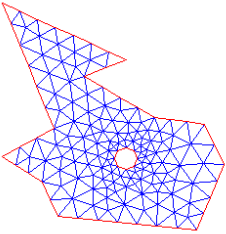
\includegraphics[width=0.34\textwidth]{assets/fig-2-1.png}
\figcaption{Fig. 2.1. \quad Example simulation region divided by an irregular triangular mesh.}
\end{figure}

The solution of the differential equation is the sum of approximate solutions found for all mesh
elements [2].
\begin{equation}
f(x,y)=\sum_{i=1}^{n}f_i(x,y). \tag{2.11}
\end{equation}
In the simplest case, the functions $f_i(x,y)$ have the form of first-degree polynomials of two
spatial variables:
\begin{equation}
f_i(x,y)=a+bx+cy. \tag{2.12}
\end{equation}
Finding the coefficients $a$, $b$, and $c$ requires solving a system of three linear equations with
three unknowns, whose coefficients are combinations of the positions $(x_{iw},y_{iw})$ of the nodes
of the element and of the solutions of the given differential equation at those points. The matrix form
of the system of equations is presented below.
\begin{equation}
\begin{bmatrix}
f_{1w}\\ f_{2w}\\ f_{3w}
\end{bmatrix}
=
\begin{bmatrix}
1&x_{1w}&y_{1w}\\
1&x_{2w}&y_{2w}\\
1&x_{3w}&y_{3w}
\end{bmatrix}
\begin{bmatrix}
a\\ b\\ c
\end{bmatrix}. \tag{2.13}
\end{equation}
Thus the matrix of coefficients $a$, $b$, and $c$ is given by
\begin{equation}
\begin{bmatrix}
a\\ b\\ c
\end{bmatrix}
=
\begin{bmatrix}
1&x_{1w}&y_{1w}\\
1&x_{2w}&y_{2w}\\
1&x_{3w}&y_{3w}
\end{bmatrix}^{-1}
\begin{bmatrix}
f_{1w}\\ f_{2w}\\ f_{3w}
\end{bmatrix}. \tag{2.14}
\end{equation}
Numerical methods for finding the values $f_1$, $f_2$, and $f_3$ depend strictly on the type of
differential equation being solved.

\subchaptertitle{2.3. Elliptic differential equation and a method for its approximate solution}

The form of an elliptic differential equation is described by equation (2.15), where $f$ is the function
sought in the region $\Omega$, and $a$, $b$, and $c$ are coefficients of the equation.
\begin{equation}
-\nabla\cdot(c\nabla f)+af=b. \tag{2.15}
\end{equation}
The value of $f$ on the boundary of the region $\Omega$ (hereafter $\partial\Omega$) is specified by
Dirichlet conditions of type (2.16a) or Neumann conditions of type (2.16b).
\begin{align}
hf &= r, \tag{2.16a}\\
\mathbf n(c\nabla f)+qf &= g. \tag{2.16b}
\end{align}
The quantities $h$, $r$, and $q$ are successive coefficients of the equations, and $\mathbf n$ is the
normal vector to $\partial\Omega$. In the case of the two-dimensional vector wave equation, boundary
conditions are chosen so as to avoid, as well as possible, reflections at the boundary of the simulation
region. This problem can largely be avoided by using a PML (perfectly matched layer), which is
discussed in section 2.4.

Equation (2.15) is multiplied by a test function $v$ and both sides are integrated over the region
$\Omega$, yielding equation (2.17), and is then integrated by parts, bringing it to the form shown
in (2.18) [3,4].
\begin{align}
\int_\Omega\left((-\nabla\cdot c\nabla f)v+auf\right)\,dx &= \int_\Omega bv\,dx, \tag{2.17}\\
\int_\Omega\left((c\nabla f)\cdot\nabla v+afv\right)\,dx-\int_{\partial\Omega}(-qf+g)v\,ds &= \int_\Omega bv\,dx. \tag{2.18}
\end{align}
Next, the above equation is written in the so-called weak form, and its solution is called a weak
solution. One seeks functions $f$ satisfying (2.19) for all $v$.
\begin{equation}
\int_\Omega\left((c\nabla f)\cdot\nabla v+afv-bv\right)\,dx-\int_{\partial\Omega}(-qf+g)v\,ds=0. \tag{2.19}
\end{equation}
The functions $f$ and $v$ belong to the same space $V$. One must choose a finite-dimensional
subspace $V'\subset V$, whose dimension $\dim V'$ determines the number of nodes, and to which
the set of test functions $v_i$ forming the basis will belong. The dimension of $V'$ determines the
accuracy of the calculation result. The sought solution of the problem is the element of the subspace
lying closest to the weak solution in the sense of the norm $||r||$, whose form is given below.
\begin{equation}
||r||=\int_\Omega(c|f|^2+af^2)\,dx+\int_{\partial\Omega}qf^2\,ds. \tag{2.20}
\end{equation}
The function $f(x)$ can then be expanded in a series, giving the approximate solution
\begin{equation}
f(x)\approx\sum_{j=1}^{\dim V'}F_jv_j(x). \tag{2.21}
\end{equation}
Substituting the above formula into the discretized equation (2.18) gives the following system of
equations:
\begin{equation}
\begin{aligned}
\sum_{j=1}^{\dim V'}\bigg(&\int_\Omega\left((c\nabla v_j)\cdot\nabla v_j+av_jv_i\right)\,dx
+\int_{\partial\Omega}qv_jv_i\,ds\bigg)F_j \\
&=\int_\Omega bv_i\,dx+\int_{\partial\Omega}gv_i\,ds,\quad i=1,\ldots,\dim V'.
\end{aligned}
\tag{2.22}
\end{equation}
The quantity (2.23a) is called the stiffness matrix, while the quantity (2.23b) is called the mass
matrix. These names follow from the applicability of the above method to solving problems in statics.
\begin{align}
K_{i,j} &= \int_\Omega(c\nabla v_j)\cdot\nabla v_i\,dx, \tag{2.23a}\\
M_{i,j} &= \int_\Omega av_jv_i\,dx. \tag{2.23b}
\end{align}
The resulting system of equations of the form $AF=B$ gives the solutions of the elliptic differential
equation at all nodes of the mesh. More extensive information on approximate methods for finding
solutions of differential equations is presented in [3,4].

\subchaptertitle{2.4. PML boundary conditions}

A serious problem encountered when performing electromagnetic simulations is the reflection of
propagating waves from the boundaries of the simulation region, resulting from imperfections of
the boundary conditions used. This can seriously disturb the obtained results. To avoid this problem,
a nonreflecting and lossy layer, called a PML (perfectly matched layer), is introduced [5].

\begin{figure}[H]\centering
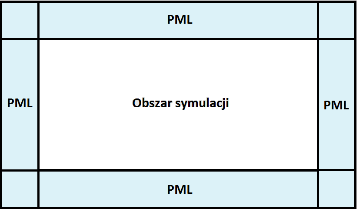
\includegraphics[width=0.56\textwidth]{assets/fig-2-2.png}
\figcaption{Fig. 2.2. \quad Schematic of a system surrounded by a PML layer.}
\end{figure}

For a normally incident wave, the condition for the absence of reflections at the interface of media is
equality of impedances, $\eta=\sqrt{\mu/\epsilon}$.
\begin{equation}
\sqrt{\frac{\mu_0\mu_1}{\epsilon_0\epsilon_1}}=\sqrt{\frac{\mu_0\mu_2}{\epsilon_0\epsilon_2}}. \tag{2.24}
\end{equation}

A generalization of this condition to oblique incidence is an artificially introduced region with specially
chosen anisotropic permittivities $\epsilon$ and permeabilities $\mu$. A PML does not belong to the region
of the considered problem and is nonphysical. Materials with properties close to those of a perfectly
matched layer can, however, be obtained in the form of multilayer structures [6]. Finally, introducing
the matrix
\begin{equation}
S=\begin{bmatrix}s^{-1}&0\\0&s\end{bmatrix}, \tag{2.25}
\end{equation}
$s=1+\alpha i$, where $\alpha$ is an arbitrarily chosen real number, the two-dimensional vector wave
equations for nonmagnetic materials in PML regions for TE and TM polarization at the horizontal
boundary of the simulation region take the forms (2.26a) and (2.26b), respectively, while in regions
at the vertical boundary they take the forms (2.27a) and (2.27b).
\begin{align}
-\nabla\cdot(S\nabla E_z)-sk_0^2\epsilon_zE_z &= 0, \tag{2.26a}\\
-\nabla\cdot(S\epsilon^{-1}\nabla H_z)-sk_0^2H_z &= 0, \tag{2.26b}\\
-\nabla\cdot(S^{-1}\nabla E_z)-sk_0^2\epsilon_zE_z &= 0, \tag{2.27a}\\
-\nabla\cdot(S^{-1}\epsilon^{-1}\nabla H_z)-sk_0^2H_z &= 0, \tag{2.27b}
\end{align}
where the operator $\nabla$ is restricted to two dimensions. These equations can also be modified for
corner regions; however, using one of the above also gives satisfactory results.

An example of the use of a perfectly matched layer is shown in Fig. 2.3. Diffraction of a TE-polarized
electromagnetic wave by a narrow slit cut in a material that is a perfect conductor was considered.
Thanks to the use of PML boundary conditions, the absence of reflections can be observed. The result
below was obtained using the FEM method.

\begin{figure}[H]\centering
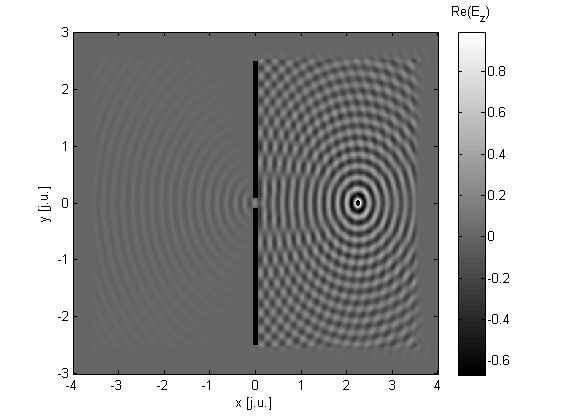
\includegraphics[width=0.58\textwidth]{assets/fig-2-3.png}
\figcaption{Fig. 2.3. \quad Diffraction of an electromagnetic wave by a narrow slit.}
\end{figure}

\subchaptertitle{2.5. Photonic crystals}

A crystal is a periodic structure composed of atoms or molecules. The arrangement of these
components defines the type of crystal lattice of the system. A characteristic property of crystals
is the possible occurrence of a so-called band gap. This means that, for certain values of energy and
momentum, an electron cannot move in such a structure. When propagation is impossible in any
direction within a specified energy range, the gap is called complete; otherwise it is called partial.
An example of a complete band gap is the band structure of semiconductors, in which it separates
the valence band from the conduction band.

The analogous structure in optics is a photonic crystal. It is a periodic structure made of dielectric
materials that differ in electric permittivity. The period of such a system is comparable with the
wavelength for which it is to perform its function. Depending on the directions of periodicity, one-,
two-, and three-dimensional crystals are distinguished.

\begin{figure}[H]\centering
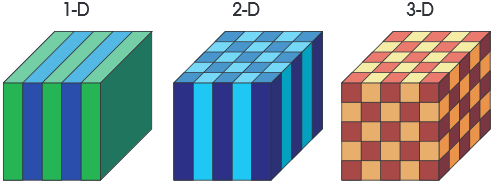
\includegraphics[width=0.66\textwidth]{assets/fig-2-4.png}
\figcaption{Fig. 2.4. \quad Schematic of one-, two-, and three-dimensional photonic crystals. Differences in
color symbolize materials with different values of electric permittivity [7].}
\end{figure}

As in ordinary crystals (or generally, in periodic media), the modes of photonic crystals have the
form of Bloch waves. It also happens that electromagnetic radiation of certain frequencies cannot
propagate in the structure. This is called a photonic band gap. If, for a given frequency range, the
gap occurs for all polarizations and propagation directions, it is called complete; otherwise it is partial.

The possibility of selective propagation of light makes it possible to create structures with interesting
optical properties, such as mirrors reflecting electromagnetic radiation in a specified wavelength
range, materials with nearly zero group velocity ("slowing" light), opposite values of group and phase
velocity (backward propagation), or materials at whose boundary negative refraction occurs. Another
possibility is the creation of waveguides based on photonic crystals. A linear defect is introduced
into the structure by removing a row or several rows of dielectric rods placed in a homogeneous
matrix. In the range of the photonic band gap, a defect mode appears, allowing the propagation of
electromagnetic radiation along the resulting waveguide. An advantage of such a structure is its much
lower loss, for example in the visible-light range, compared with metallic waveguides.

\newpage
\subchaptertitle{2.6. Diffraction gratings}

A diffraction grating is a periodic system of slits (apertures) or obstacles that causes changes in the
intensity, phase, or both of a transmitted or reflected wave. Two basic types of gratings are distinguished:
amplitude gratings and phase gratings. In the first case, light encounters alternating transparent and
opaque regions, which modulates the amplitude. In the second case, the optical path difference
resulting from corrugation of transparent elements modulates the phase. If the corrugated diffraction
grating is not completely transparent in places, both amplitude and phase modulation occur.

For a wave normally incident on a transmission grating, one can introduce the equation
\begin{equation}
\Lambda\sin\theta=m\lambda, \tag{2.28}
\end{equation}
relating the grating period $\Lambda$, the angle $\theta$ at which intensity maxima are observed, and
the wavelength $\lambda$. The integer $m$ indexes the diffraction order. The above equation can be
generalized for oblique incidence [8]:
\begin{equation}
\Lambda(\sin\theta_m-\sin\theta_i)=m\lambda. \tag{2.29}
\end{equation}
$\theta_i$ is the angle at which the wave is incident on the structure, and $\theta_m$ is the angle at
which the $m$-th diffraction order is observed.

\begin{figure}[H]\centering
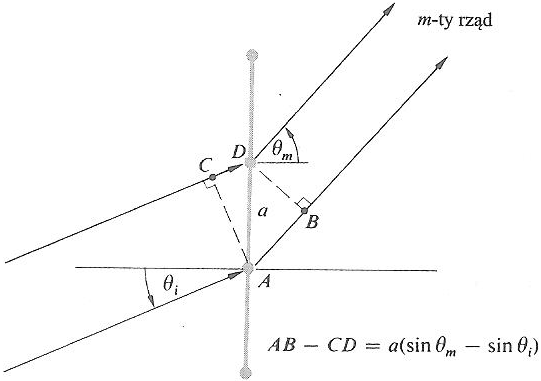
\includegraphics[width=0.64\textwidth]{assets/fig-2-5.png}
\figcaption{Fig. 2.5. \quad Schematic of oblique incidence of electromagnetic radiation on a transmission
diffraction grating [8].}
\end{figure}

The above relations show that, for a given wavelength and a specified grating period, there is a finite
number of real diffraction orders. It is known that, in two dimensions,
\begin{equation}
k_x^2+k_y^2=k_0^2n^2, \tag{2.30}
\end{equation}
where $n$ is the refractive index of the external medium. At the same time, for a wave diffracted by
a system periodic in the $x$ direction, the vector $k_x$ is conserved up to multiples of $2\pi/\Lambda$:
\begin{equation}
k_x^{(0)}=k_x^{(i)}+\frac{2\pi m}{\Lambda}, \tag{2.31}
\end{equation}
where the index (i) corresponds to the incident wave and (0) to the wave leaving the grating. Thus,
for large $m$, $|k_x^{(0)}|>k_0n$, and therefore $k_y^{(0)}=\sqrt{k_0^2n^2-(k_x^{(0)})^2}$ takes imaginary
values. One then deals with evanescent, exponentially decaying diffraction orders.

In the case of diffraction gratings composed of several systems of elements with different periods,
the number of real diffraction orders depends on the direction from which such a structure is
illuminated. This is shown in the simulations whose results are presented in section 3.2.

\newpage
\chaptertitle{Chapter 3. Simulation results}

This chapter presents simulations carried out independently. The finite element method was used
(the "PDE Toolbox" package by MathWorks), and its results were compared with selected results
obtained using the finite difference time domain method [9] (the MEEP program [10]). To find the
band structure of photonic crystals, the MPB -- MIT Photonic Bands program [11], based on the
plane wave method, was used.

\subchaptertitle{3.1. Propagation of light in photonic crystals}

Two-dimensional photonic crystals with two lattice types were considered: square and triangular.

\begin{figure}[H]\centering
\begin{minipage}{0.33\textwidth}\centering
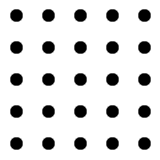
\includegraphics[width=0.85\linewidth]{assets/fig-3-1a.png}
\end{minipage}\hspace{0.8cm}
\begin{minipage}{0.33\textwidth}\centering
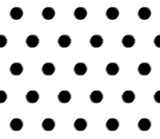
\includegraphics[width=0.85\linewidth]{assets/fig-3-1b.png}
\end{minipage}
\figcaption{Fig. 3.1. \quad Schematics of two-dimensional crystal lattices: square (left) and
triangular (right).}
\end{figure}

Each black element in the above figure is a dielectric rod of radius $0.2a$ (where $a$ is the lattice
period) and $n_1=1.7865$, which is the refractive index of sapphire (Al$_2$O$_3$) for electromagnetic
radiation of wavelength 400 nm [12]. The rods were placed in a material with $n_2=1$, which with
good accuracy can be taken as the refractive index of air (in fact, it is the refractive index of vacuum).

Band structures were determined for a specified, previously defined refractive index. However, because
of dispersion, this index actually changes with wavelength [13]. Therefore, modeling was performed
for the previously mentioned wavelength of 400 nanometers, while changes in frequency (expressed
in dimensionless units $2\pi c/a$) were introduced by modifying the size of the crystal, and in particular
the value of $a$.

Fig. 3.2 shows the band diagram obtained for TE- and TM-polarized light in a photonic crystal with
a square lattice. For neither of these polarizations is a photonic band gap observed. This means that
electromagnetic radiation can propagate in such a structure for all frequencies for which the band
structure was determined. By cutting out one row of dielectric rods, a waveguide was obtained, and
then the propagation of light in it was simulated using the finite element method.

\begin{figure}[H]\centering
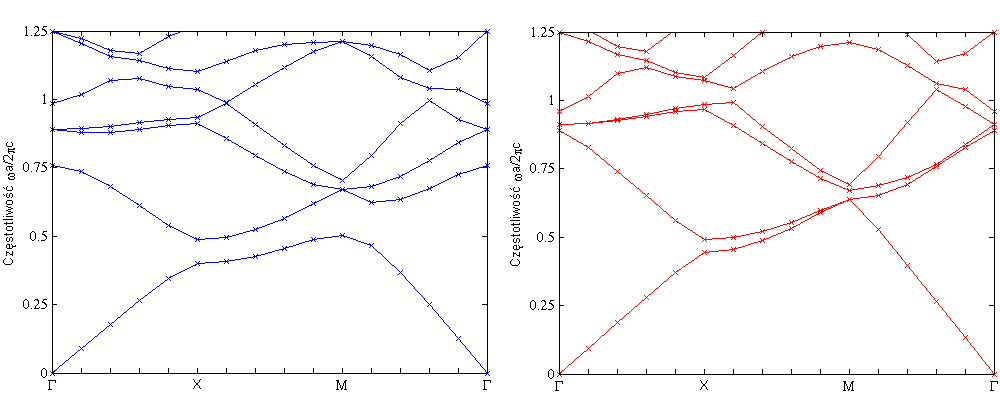
\includegraphics[width=0.88\textwidth]{assets/fig-3-2.png}
\figcaption{Fig. 3.2. \quad Band structure of a crystal with a square lattice, TE polarization (left plot),
TM polarization (right plot).}
\end{figure}

Figs. 3.3--3.5 show the simulation results obtained for the above case for three different radiation
frequencies. In each case, the electromagnetic field was introduced into the system using a hard
source located near the considered structure. The simulations were performed for TE polarization.
Both the real part of the wave field $E_z$ and its phase are shown. As illustrated schematically in
Fig. 2.2, the outer region of the simulation is a PML. All simulations of electromagnetic radiation
propagation were performed using the FEM method unless otherwise indicated in the caption.

\twopanel{assets/fig-3-3a.png}{assets/fig-3-3b.png}{Fig. 3.3. \quad Propagation of an EM wave in a photonic crystal with a square lattice and a linear defect.}{a) Instantaneous field $E_z$, b) phase of the field $E_z$ for $\omega=0.20\,2\pi c/a$.}

\twopanel{assets/fig-3-4a.png}{assets/fig-3-4b.png}{Fig. 3.4. \quad Propagation of an EM wave in a photonic crystal with a square lattice and a linear defect.}{a) Instantaneous field $E_z$, b) phase of the field $E_z$ for $\omega=0.45\,2\pi c/a$.}

\twopanel{assets/fig-3-5a.png}{assets/fig-3-5b.png}{Fig. 3.5. \quad Propagation of an EM wave in a photonic crystal with a square lattice and a linear defect.}{a) Instantaneous field $E_z$, b) phase of the field $E_z$ for $\omega=0.70\,2\pi c/a$.}

The above simulations confirm that, for the selected frequencies, light propagates in the structure
under consideration.

Analogously, the band structure of a photonic crystal with a triangular lattice was determined and
is shown in Fig. 3.6. For TE polarization, a band gap is observed in the frequency range $\omega a/2\pi c$
from about 0.48 to about 0.55. It is marked in yellow. In the case of TM polarization, no gap was
observed. Therefore, as for the square lattice, the simulations focused only on the first of these
polarizations.

\begin{figure}[H]\centering
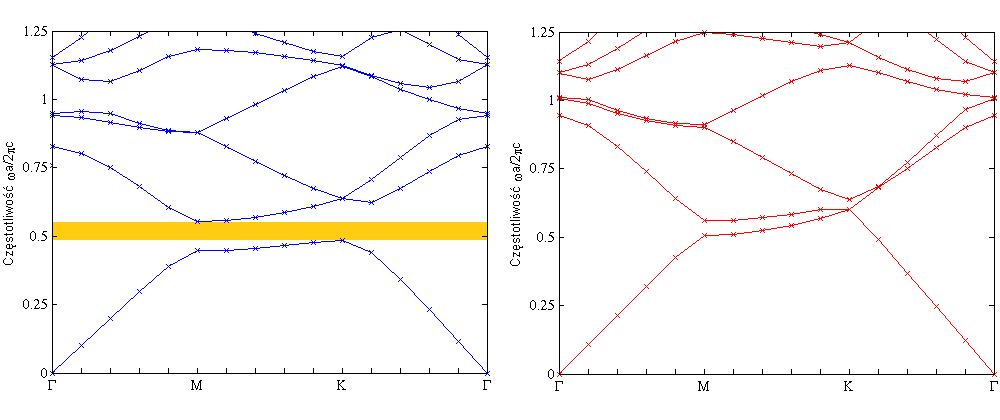
\includegraphics[width=0.88\textwidth]{assets/fig-3-6.png}
\figcaption{Fig. 3.6. \quad Band structure of a crystal with a triangular lattice, TE polarization (left plot),
TM polarization (right plot).}
\end{figure}

Determining the band structure for a waveguide formed by removing one row of rods indicates the
formation of a guided mode (highlighted in green) lying inside the band gap of the crystal, as can
be seen in the figure below.

\begin{figure}[H]\centering
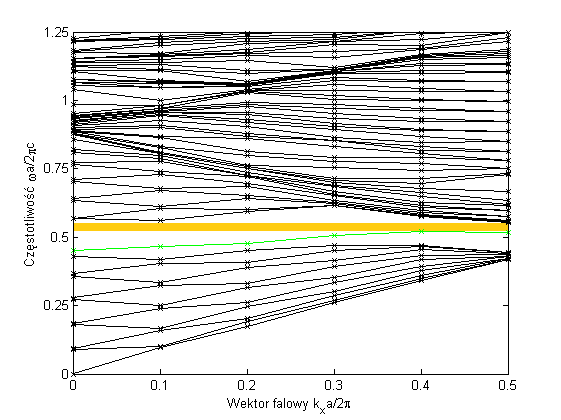
\includegraphics[width=0.66\textwidth]{assets/fig-3-7.png}
\figcaption{Fig. 3.7. \quad Band structure of a crystal with a triangular lattice and a linear defect.}
\end{figure}

Figs. 3.8--3.10 show the propagation in such a waveguide of radiation with frequencies $\omega a/2\pi c$
equal to 0.20, 0.45, and 0.70, respectively. They do not lie in the band-gap range, but are intended
to illustrate differences between the results obtained for the square and triangular lattices.

\twopanel{assets/fig-3-8a.png}{assets/fig-3-8b.png}{Fig. 3.8. \quad Propagation of an EM wave in a photonic crystal with a triangular lattice and a linear defect.}{a) Instantaneous field $E_z$, b) phase of the field $E_z$ for $\omega=0.20\,2\pi c/a$.}

\twopanel{assets/fig-3-9a.png}{assets/fig-3-9b.png}{Fig. 3.9. \quad Propagation of an EM wave in a photonic crystal with a triangular lattice and a linear defect.}{a) Instantaneous field $E_z$, b) phase of the field $E_z$ for $\omega=0.45\,2\pi c/a$.}

Fig. 3.8, obtained for a low frequency, that is, a large wavelength, is consistent with the result
obtained for the same input wave when considering the square-lattice system. One can conclude
that, in this case, the crystal structure does not affect the way light propagates. This confirms the
fact that the lattice constant of a photonic crystal should be comparable with the wavelength with
which the crystal is to interact, as mentioned in section 2.5. Only for higher frequencies do differences
in propagation begin to be noticeable. In this thesis, however, light propagation was not modeled for
very high frequencies, that is, for wavelengths much smaller than the lattice constant of the photonic
crystal.

\twopanel{assets/fig-3-10a.png}{assets/fig-3-10b.png}{Fig. 3.10. \quad Propagation of an EM wave in a photonic crystal with a triangular lattice and a linear defect.}{a) Phase of the field $E_z$, b) instantaneous field $E_z$ for $\omega=0.70\,2\pi c/a$.}

Next, modeling was performed for an electromagnetic wave with a frequency from the guided-mode
range. It is easy to see that light propagates mainly along the linear defect, and essentially no
propagation in other directions is observed. This is shown below.

\twopanel{assets/fig-3-11a.png}{assets/fig-3-11b.png}{Fig. 3.11. \quad Propagation of an EM wave in a photonic crystal with a triangular lattice and a linear defect.}{a) Phase of the field $E_z$, b) instantaneous field $E_z$ for $\omega=0.50\,2\pi c/a$.}

For comparison, the simulation was repeated using the finite difference time domain method. A
comparable result was obtained. Small differences may result from the fact that the calculated
quantity is the instantaneous field, and also from the fact that a different type of source was used
in MEEP, not a hard source, as well as a different input amplitude. There is no doubt, however, that
the results obtained by the FEM and FDTD methods agree.

\begin{figure}[H]\centering
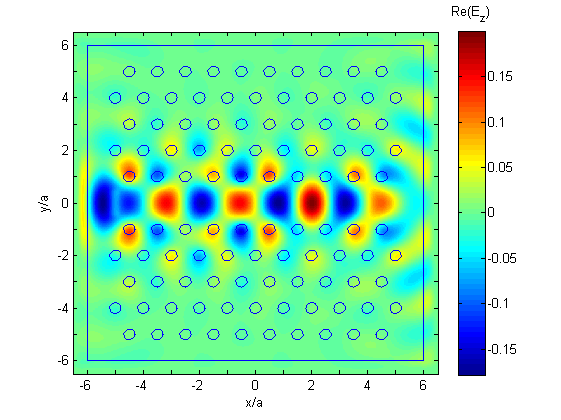
\includegraphics[width=0.48\textwidth]{assets/fig-3-12.png}
\figcaption{Fig. 3.12. Propagation of an EM wave in a photonic crystal with a triangular lattice and a linear defect.
Instantaneous field $E_z$ for $\omega=0.50\,2\pi c/a$. Simulation performed using the FDTD method.}
\end{figure}

Finally, for a frequency lying inside the band gap (the value $\omega a/2\pi c=0.538$ was
chosen), a decay of the wave amplitude with increasing distance from the source is observed. The
simulation results obtained by the finite element method are therefore consistent with the ranges of
the photonic band gap and guided mode determined by the MPB program.

\twopanel{assets/fig-3-13a.png}{assets/fig-3-13b.png}{Fig. 3.13. \quad Propagation of an EM wave in a photonic crystal with a triangular lattice and a linear defect.}{a) Instantaneous field $E_z$, b) phase of the field $E_z$ for $\omega=0.538\,2\pi c/a$.}

As in the case of simulations performed for guiding light in a localized defect mode, the finite
difference time domain method gives almost identical results to the finite element method for a
frequency lying inside the photonic band gap.

\begin{figure}[H]\centering
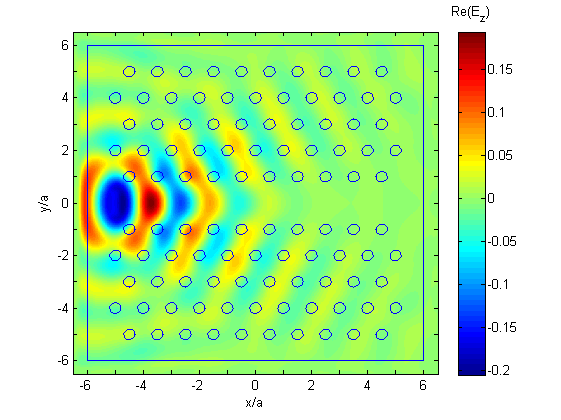
\includegraphics[width=0.48\textwidth]{assets/fig-3-14.png}
\figcaption{Fig. 3.14. Propagation of an EM wave in a photonic crystal with a triangular lattice and a linear defect.
Instantaneous field $E_z$ for $\omega=0.538\,2\pi c/a$. Simulation performed using the FDTD method.}
\end{figure}

\newpage
\subchaptertitle{3.2. Diffractive elements with double periodicity}
\begingroup\small

Diffractive elements with double periodicity are systems built from two subwavelength gratings with
different periods. According to what was presented in chapter 2.6, the number of real diffraction
orders depends on the direction from which light is incident on such a structure. At the same time,
asymmetric transmission of electromagnetic radiation and removal of the zeroth diffraction order can
be observed [14].

In the simulations carried out for this chapter, systems made successively of a perfect conductor,
chromium, gold, and silver were considered. Their schematic is shown in the figure below.

\begin{figure}[H]\centering
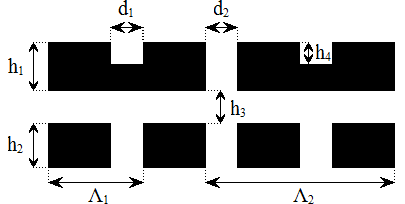
\includegraphics[width=0.58\textwidth]{assets/fig-3-15.png}
\figcaption{Fig. 3.15. \quad Schematic of a diffraction grating with double periodicity.}
\end{figure}

The dimensions used were, successively: $2\Lambda_1=\Lambda_2=533$ nm; $d_1=d_2=89$ nm;
$h_1=h_2=127$ nm; $h_3=89$ nm; $h_4=63.5$ nm.

The following simulations were performed using the FEM method for an electromagnetic wave of
wavelength 400 nm. TM polarization was used. The electric permittivity values for the metals
considered are listed in the table.

\begin{table}[H]\centering
\caption*{\small Table 3.1 \quad Electric permittivities of selected metals for waves of wavelength 400 nm [15].}
\begin{tabular}{|p{0.29\textwidth}|p{0.29\textwidth}|p{0.29\textwidth}|}
\hline
& \centering $\epsilon_1$ & \centering\arraybackslash $\epsilon_2$\\
\hline
Silver & -4.422 & 0.210\\
\hline
Gold & -1.658 & 5.735\\
\hline
Chromium & -4.055 & 11.480\\
\hline
\end{tabular}
\end{table}

The permittivities $\epsilon_1$ and $\epsilon_2$ contribute to the complex electric permittivity
\begin{equation}
\tilde\epsilon=\epsilon_1+i\epsilon_2. \tag{3.1}
\end{equation}
Five hard sources, whose centers were located above the slits of the grating, were used to emit
spherical waves.

Fig. 3.16 shows the transmission of light through a structure in which the diffraction grating is made
of a perfect conductor. For an electromagnetic wave incident from above, two diffraction orders are
visible: -1 and 1. For incidence from the other side, only the zeroth diffraction order is observed,
which is consistent with the theory presented in section 2.6.

\newpage
\twopanel{assets/fig-3-16a.png}{assets/fig-3-16b.png}{Fig. 3.16. \quad Perfect-conductor grating,}{a) incidence from above, b) incidence from below.}

The use of spherical waves caused a slight deviation of the zeroth diffraction order from the angle
0° with respect to the normal to the direction of periodicity of the structure. This follows from
formula 2.29.

Comparable results were obtained for simulations performed for chromium. Increased transmission
is observed compared with the perfect conductor, but one can conclude that, of the three metals
considered, this one is the most similar to it.

\twopanel{assets/fig-3-17a.png}{assets/fig-3-17b.png}{Fig. 3.17. \quad Chromium grating,}{a) incidence from above, b) incidence from below.}

When gold is used, enhanced transmission through the structure is observed. Penetration of light
into the elements of the system can be noticed. For the simulation in which the electromagnetic wave
was incident from above, three diffraction orders can clearly be seen.

\newpage
\twopanel{assets/fig-3-18a.png}{assets/fig-3-18b.png}{Fig. 3.18. \quad Gold grating,}{a) incidence from above, b) incidence from below.}

Interesting results were obtained for a system made of silver, for which the transmission of
electromagnetic radiation turned out to be residual regardless of the direction of incidence.

\twopanel{assets/fig-3-19a.png}{assets/fig-3-19b.png}{Fig. 3.19. \quad Silver grating,}{a) incidence from above, b) incidence from below.}

\endgroup
\newpage
\chaptertitle{Chapter 4. Conclusions}

For the purposes of this thesis, a series of simulations concerning the propagation of light in photonic
crystals and in diffractive elements with double periodicity were carried out. The work was based
on the finite element method.

In the case of photonic crystals, the first step was to determine their band structure, which was
possible with the aid of the plane wave method, applicable to optical periodic systems. Two types
of lattice were considered: square and triangular. The behavior of light of a specified wavelength
was modeled by changing the size of the photonic crystal. It was checked that, in some structures of
this type, for certain wave polarizations and in a specified frequency range, a photonic band gap is
present. It was also shown that, by introducing defects, efficient guiding of light with a frequency
lying inside such a gap becomes possible through the formation of a defect mode. Selected results
were then compared with simulations performed using the finite difference time domain method.

For diffractive elements with double periodicity it was shown that the number of observed real
diffraction orders generally depends on the direction of illumination of the structure. It was also
shown that the material from which the system is made has a significant influence on its operation.
For this purpose, modeling was performed for a perfect conductor, chromium, gold, and silver. Many
similarities were noted for the perfect conductor and chromium; in the case of gold, enhanced
transmission of electromagnetic radiation was observed, while in the case of silver it was almost not
observed at all.

It was shown that the finite element method is a useful tool that can be used to design optical
systems with characteristic properties. The auxiliary use of tools such as the plane wave method
significantly facilitated the simulation of differences in the behavior of light depending on the size
of the structure or the material from which it is made. It was demonstrated that combining several
techniques for determining the properties of a structure is extremely important in the effective design
of new materials. This makes it possible to easily optimize optical elements and also creates an
opportunity for the effective design of new, more complex systems.

\newpage
\chaptertitle{Bibliography}

\begin{enumerate}
\renewcommand{\labelenumi}{[\arabic{enumi}]}
\item D. J. Griffiths, \textit{Fundamentals of Electrodynamics}, 2nd ed., Wydawnictwo Naukowe PWN (2005), pp. 354-366
\item M. N. O. Sadiku, \textit{Numerical Techniques in Electromagnetics}, 2nd ed., CRC Press (2000), chapter 6
\item C. Johnson, \textit{Numerical Solution of Partial Differential Equations by the Finite Element Method}, Cambridge University Press (1987)
\item R. E. Bank, \textit{PLTMG A Software Package for Solving Elliptic Partial Differential Equations}, User's Guide 6.0, Society for Industrial and Applied Mathematics, Philadelphia, PA (1990)
\item J.P. Berenger, \textit{Perfectly Matched Layer (PML) for Computational Electromagnetics}. Morgan and Claypool, Los Altos (2007)
\item A. Pastuszczak, M. Stolarek, T. J. Antosiewicz and R. Kotyński, \textit{Multilayer metamaterial absorbers inspired by perfectly matched layers}, Optical and Quantum Electronics, DOI 10.1007/s11082-014-9986-z (2014)
\item J. D. Joannopoulos, S. G. Johnson, J. N. Winn and R. D. Meade, \textit{Photonic Crystals, Molding the Flow of Light}, 2nd ed., Princeton University Press (2008), p. 4
\item E. Hecht, \textit{Optics}, 1st ed., Wydawnictwo Naukowe PWN (2005), pp. 479-482
\item A. Taflove, S. C. Hagness, \textit{Computational Electrodynamics: The Finite-Difference Time-Domain Method}, 3rd ed., Artech House (2005)
\item A. F. Oskooi, D. Roundy, M. Ibanescu, P. Bermel, J. D. Joannopoulos and S. G. Johnson, \textit{MEEP: A flexible free-software package for electromagnetic simulations by the FDTD method}, Computer Physics Communications \textbf{181}, pp. 687--702 (2010)
\item S. G. Johnson and J. D. Joannopoulos, \textit{Block-iterative frequency-domain methods for Maxwell's equations in a planewave basis}, Optics Express \textbf{8}, pp. 173-190 (2001)
\item I. H. Malitson and M. J. Dodge. \textit{Refractive Index and Birefringence of Synthetic Sapphire}, J. Opt. Soc. Am. \textbf{62}, 1405 (1972)
\item B. E. A. Saleh and M. C. Teich, \textit{Fundamentals of Photonics}, 2nd ed., Wiley-Interscience (2007), pp. 173-174
\item M. Stolarek, D. Yavorskiy, R. Kotyński, C. J. Zapata Rodríguez, J. Łusakowski and T. Szoplik, \textit{Asymmetric transmission of terahertz radiation through a double grating}, Optics Letters \textbf{38}, pp. 839-841 (2013)
\item P. B. Johnson and R. W. Christy. \textit{Optical Constants of the Noble Metals}, Physical Review \textbf{B 6}, pp. 4370-4379 (1972)
\end{enumerate}

\end{document}
